\chapter{Materials and Methods}\label{chap:method}
This chapter describes the tools and measurement instruments used throughout the empirical studies described in later chapters. Specifically, the NAO robot and Sandtray touchscreen are introduced, with an explanation of how they operate in tandem to deliver the learning content in interactions. Standard \gls{immediacy} metrics and the `child-friendly' versions developed for use with robots in this research are also discussed. Study specific tests and materials will be described in the relevant later chapters.

%%%%%%%%%%%%%%%%%%%%%%%%%%%%%%%%%%%%%%%%%%%%%%%%%%%%%%%%%%%%
\section{The NAO Robot}\label{sec:method-nao}
The Aldebaran NAO robot is a 58cm tall humanoid robot which is used as the sole robotic platform throughout this research (Figure \ref{fig:ch3_nao}). The robot is available to researchers, developers and educational institutions. The robot (or NAO) has 25 degrees of freedom and a variety of sensors, including microphones, touch sensors and cameras. Additionally, two speakers are mounted in the head of the robot to play sound. The eyes of the robot contain an array of Light Emitting Diodes (LEDs) which can change colour.

\begin{figure}[ht]
    \centering
    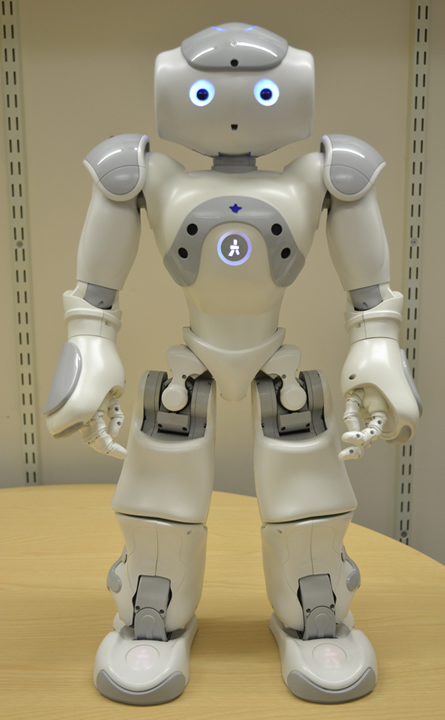
\includegraphics[width=0.5\textwidth]{images/ch3_nao.jpg}
    \caption{The Aldebaran NAO used in the majority of the evaluations throughout this thesis.}
    \label{fig:ch3_nao}
\end{figure}

Two different hardware versions of the NAO robot were used during this research: a v3 H25 body with a v3.3 and a v4 head. Both versions of the head incorporate a custom Linux distribution with the \textit{NaoQi} operating system acting as an interface to the programmer. The versions of NaoQi used here (1.12.x and 1.22.x) include Nuance speech recognition and a Text-To-Speech engine provided by Acapela.

The NAO robot is particularly suited for interaction with children due to to its small size and approachable appearance \citep{shamsuddin2012initial}. Humanoid robots also benefit from having modalities that map to the human body, thus enabling implementation of social behaviour based on human models. Principles from human-human research can also be more readily transferred, providing a possible theoretical starting point for investigation or development of research questions.

The \textit{Universal Real-Time Behavior} (Urbi) middleware \citep{baillie2008urbi} was installed on the robot in addition to the standard packages. Urbi is specialised for robot control, providing many high-level orchestration functionalities, easing real-time multimodal behaviour control. A convenient scripting language (UrbiScript) is used for programming the robot. UrbiScript closely resembles C++, but has additional operators to determine whether lines, or blocks, of code should be executed in serial or parallel, synchronously or asynchronously. Urbi offers the ability to perform offboard processing, but all robot control and communication to external devices in this research was performed through UrbiScript running directly on the robot. Urbi versions 2.7.5 and 3.0 were used during this project; they are tied to NaoQi versions 1.12.x and 1.22.x respectively.

%%%%%%%%%%%%%%%%%%%%%%%%%%%%%%%%%%%%%%%%%%%%%%%%%%%%%%%%%%%%
\section{The Sandtray Touchscreen}\label{sec:method-sandtray}
The \textit{Sandtray} touchscreen, developed by \cite{baxter2012touchscreen} to constrain \acrshort{hri} and provide a shared workspace for both the human and robot, is used in the majority of the studies for this research. Two different versions of the Sandtray have been used throughout this research (Figures \ref{fig:ch3_old_sandtray} and \ref{fig:ch3_new_sandtray}). Both versions consist of a large touchscreen mounted horizontally. The first version had a 26 inch screen at a height of 30 centimetres above the floor, and the second version had a 27 inch all-in-one touchscreen computer mounted 26 centimetres above the floor. This is an ideal height for the NAO robot to convincingly appear to manipulate items on the screen, and is also easy for children to use when seated on the floor. When using the first Sandtray version, the robot would stand on a small platform to reduce the height difference to the desired 26 centimetres. The first version also required a separate computer to display on the touchscreen; to this end, a laptop was used and hidden in the housing below the screen.

\begin{figure}[ht]
    \centering
    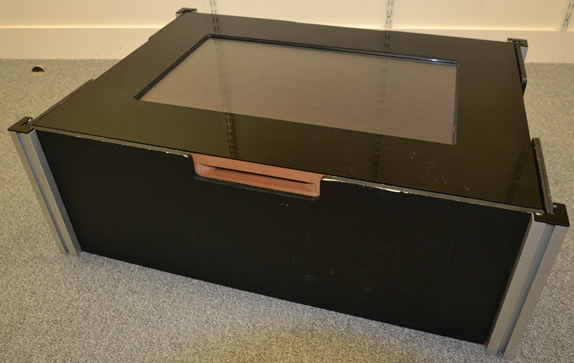
\includegraphics[width=0.5\textwidth]{images/ch3_old_sandtray.jpg}
    \caption{Version 1 of the Sandtray touchscreen used in experimental evaluations. A laptop is stored within the wooden housing to run the software, with the touchscreen used as a display.}
    \label{fig:ch3_old_sandtray}
\end{figure}

\begin{figure}[ht]
    \centering
    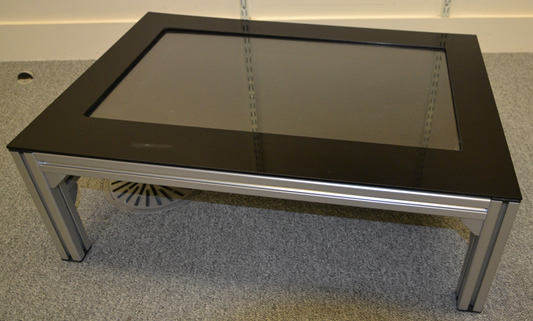
\includegraphics[width=0.5\textwidth]{images/ch3_new_sandtray.jpg}
    \caption{Version 2 of the Sandtray touchscreen used in experimental evaluations. This version is much improved, with a sturdier yet smaller construction, larger screen, lighter weight, and built-in computer.}
    \label{fig:ch3_new_sandtray}
\end{figure}

The Sandtray runs a Windows operating system (versions 7, 8, and 8.1 at varying times), with a custom software application. This application has two-way communication with an Urbi server running on the robot. Communication between the touchscreen software and the robot is performed through socket connections over a wireless network, where encoded strings are passed with payloads, such as commands to move images on screen. An early version of the software was written in C++ with DirectX and allowed two-category sorting games to played on screen. This application was later re-written with extended functionality (including the removal of limits on the number of categories that could be used) using the Qt C++ libraries (Qt SDK version 4.8.5). The software allows simple loading of different sets of images, so the same control architecture can be used across different learning contexts such as mathematics and language learning.

Using a touchscreen as a mediator in the interaction between the child and the robot brings about many benefits. In physical realms, there are objects that are too big for the robot to grip, and gripping can be a computationally heavy (and time-expensive) process; the touchscreen acts as a shared workspace where the child and the robot have equal ability at manipulation \citep{baxter2012touchscreen}. The touchscreen also acts as a focal point in the interaction, typically not only constraining the child's verbal behaviour \citep{kennedy2013constraining}, but their nonverbal behaviour as well. The use of the screen reduces the possible space where a child might be (as they will be within touching distance of the screen, on the opposite side to the robot). This significantly reduces complexity for tasks such as gaze detection and estimation \citep{lemaignan2016real}. For the child, the touchscreen interface is intuitive for children to use, and means that they can interact on screen without requiring proficiency in the use of traditional computer input methods like keyboards and mice \citep{park2013providing}.

%%%%%%%%%%%%%%%%%%%%%%%%%%%%%%%%%%%%%%%%%%%%%%%%%%%%%%%%%%%%
\section{The Microsoft Kinect}\label{sec:method-kinect}
In some experiments, the Sandtray hardware setup was extended with a Microsoft Kinect for Windows (Kinect v1). The Kinect was added to the hardware setup with a purpose built mount, that was a measured distance from the robot (Figure \ref{fig:ch3_sandtray_kinect}). As a result, the Kinect is not likely to move during interactions and as distances to the robot are known, the matrix transformations to translate and rotate the camera view to the frame of the robot can be executed reliably. The Kinect data stream is activated and managed by an application (developed by the author) that runs on the touchscreen (underneath the game software) and communicates with the Urbi server running on the robot.

\begin{figure}[ht]
   \centering
   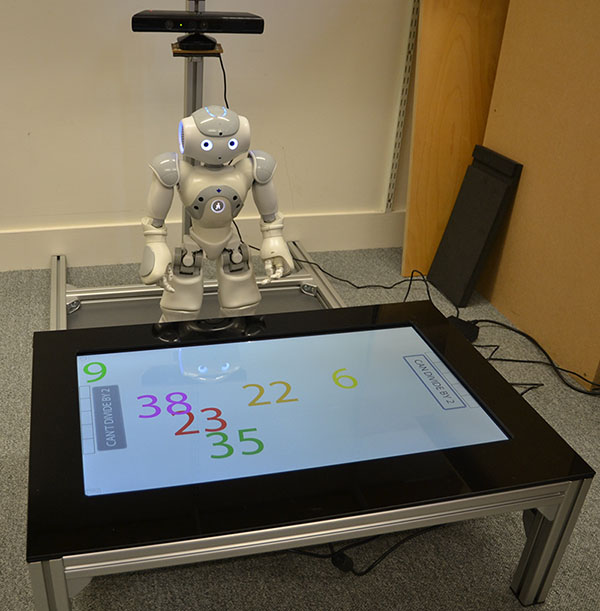
\includegraphics[width=0.7\textwidth]{images/ch3_sandtray_kinect.jpg}
   \caption{Version 2 of the Sandtray touchscreen used in experimental evaluations, with the Microsoft Kinect hardware extension. The Kinect is mounted on an additional lightweight metal frame, at a fixed distance from the robot. The robot stands with a raised rectangle on the base board. This board helps with robot stability (it allows the feet to slide more easily than the carpets often present in evaluation environments), and prevents the robot from turning away from the children when performing gestures (a common problem without fixing the feet in place).}
   \label{fig:ch3_sandtray_kinect}
\end{figure}

The Kinect application was written in Microsoft Visual Studio 2010, using the Microsoft Kinect SDK v1.7, in C\#.Net (Figure \ref{fig:ch3_kinect_cruncher}). The skeleton stream is used to select the nearest skeleton and track the head position of this skeleton. This position is rotated and translated to the robot frame of reference. Using the depth information and the head direction vector, it is calculated as to where this vector would intersect the plane of the robot. If this intersection is within a 12cm area around the robot's head, then the skeleton can be considered to be looking at the robot. The application provides events to the robot when particular actions occur (such as a new skeleton being tracked), and can be queried by the robot if particular information is required at a given time. The code running on the robot decides how to act upon this information, for instance, it may be appropriate to actively return the gaze. Simultaneously, the Kinect application logs all activity to the local Sandtray machine with a 1 second resolution, such that further post-hoc analysis can be performed when necessary. All major elements of the application are executed in separate threads so that communication and logging can occur asynchronously, maximising the tracking frame rate.
%TODO put Kinect code on GitHub and link here??

\begin{figure}[ht]
    \centering
    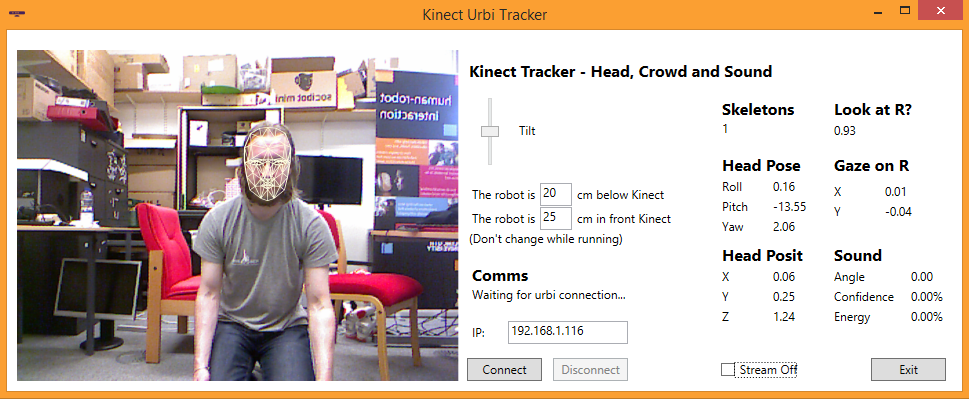
\includegraphics[width=1.0\textwidth]{images/ch3_kinect_software.png}
    \caption{Microsoft Kinect application used to process data from the Kinect sensor and to communicate with the Urbi server running on the robot. This figure shows the Kinect with the visualisation of the camera stream on, but this is turned off when evaluations are running as the application cannot be seen, and turning off the visual rendering substantially reduces CPU load.}
    \label{fig:ch3_kinect_cruncher}
\end{figure}

%%%%%%%%%%%%%%%%%%%%%%%%%%%%%%%%%%%%%%%%%%%%%%%%%%%%%%%%%%%%
\section{Robot Behaviour Generation}\label{sec:method-behave}
Despite evidence for the benefits of certain social cues (explored in detail in Section \ref{sec:background-behave}), it is still unclear precisely what can trigger learning in humans \citep{vanlehn2003only}. Additionally, descriptions of social behaviours used when teaching are often not at the resolution required by social roboticists for development and implementation. As such, there is a need to explore what social behaviour a robot should employ when tutoring in order to elicit maximal learning gains from a human interactant.

Different approaches have been adopted within the \acrshort{hri} research community, and two different approaches have been applied in this research. The first approach taken is to use a human as a model for social behaviour, for example \cite{sharma2013communicating}. It is assumed that a human is naturally social, and can provide a target behaviour to implement on a social robot. By observing a human conducting the task that the robot must complete, annotations can be made (with more accurate video coding if the interaction is filmed) and a behaviour can be derived. This approach is used in Chapters \ref{chap:embodiment} and \ref{chap:socasoc} of this thesis.

An alternative approach is to derive social behaviour from the \acrshort{hhi} literature, as in \cite{szafir2012pay}. While there are many task and context specific aspects of behaviour that cannot be derived purely from the literature, broad guidelines can be created, as shown in Section \ref{sec:background-behave}. In this case, nonverbal and \gls{verbalimm} guidelines are used to generate robot social behaviour in Chapters \ref{chap:validation}, \ref{chap:nviexperiment} and \ref{chap:verbal}.

One field of research that could also be considered as a source of information for robot behaviour is that of \acrshort{its} and Artificial Intelligence in Education \acrshort{aied} \citep{freedman2000links}. This field has been active for much longer than \acrshort{hri} and has considered challenges in instructional design in detail \citep{vanlehn2006behavior}. However, these solutions often focus on the educational aspects of tutoring, with less regard for social behaviour. This becomes a greater consideration when a social robot is used due to the increased social presence of the interacting character. Even within this literature, there are still warnings that tasks need to be developed based on a model of the intended audience \citep{murray1999authoring}. A recent call within the \acrshort{aied} community has been to switch away from traditional computers and to adopt robots as an educational platform, but the challenges (and importance) of social behaviour are seemingly not yet recognised \citep{timms2016letting}. As such, the research conducted as part of this thesis cannot draw as much as would be desired from the \acrshort{its} field due to the greater focus on social behaviour here. Tasks have followed the principle described in the \acrshort{its} literature (designing for the intended audience), but have not been re-used from the \acrshort{its} literature -- in part because appropriate tasks could not be established from \acrshort{its} for the audience and topics under consideration here.

Section \ref{sec:background-sync} indicated the importance of considering social cues in context. This means not just in the learning scenario, but also with respect to one another. Considering social cognition to be the simultaneous processing of a range of social cues as a single percept means that varying individual cues and trying to make conclusions about their use when combined with other cues and contexts is an inappropriate method \citep{zaki2013cue}. It follows that a measure which considers the combination of social cues and their interactions with one another, such as \gls{immediacy} \citep{mehrabian1968some}, is best suited for evaluating correlations in response to social behaviour.

%%%%%%%%%%%%%%%%%%%%%%%%%%%%%%%%%%%%%%%%%%%%%%%%%%%%%%%%%%%%
\section{Video Coding}\label{sec:method-vidcode}
In order to characterise both robot and child social behaviour, one technique often used in the \acrshort{hri} literature is to manually video code specific behavioural instances \citep{kahn2003coding,moshkina2014social,zaga2015effect}. The aim is to be able to quantify particular behaviours of interest by specifying when they occur, and for how long. For instance, a common social behaviour to code would be human gaze. A number of pertinent categories could be selected for this purpose, such as `towards robot', `towards touchscreen', and `other'. Following the coding process, the number of instances and amount of time that each of these behaviours occurred can then be calculated. Additionally, if multiple behaviours are coded, then correlations and patterns between the behaviours can also be investigated. For example, it may be the case that the human looks at the robot each time the robot moves. This type of analysis can be used to reveal such effects.

The coding process is often performed manually for high accuracy and reliability. To provide further confidence in the coding objectivity, multiple coders are often used, with their coding cross-referenced to verify inter-coder agreement. This is usually done through a statistical measure such as Cohen's Kappa \citep{baxter2013emergence}. To ensure that the coding process is consistent and accurate, a coding manual is commonly used and provided to all coders. An example of an extensive coding manual can be seen in \citep{kahn2003coding}, with a further example of the manual provided to coders for studies in this work in Appendix \ref{app:codingmanual}\footnote{Please note that this manual is based on the work of Paul Baxter as part of the \acrshort{alize} project and was just extended by the author to include further details specific to the study under investigation}.

For the video coding performed as part of this thesis, a free, cross-platform video annotation software called ANVIL was used \citep{kipp2001anvil}, available online: \url{http://www.anvil-software.org/}. Many alternatives are available, but access to expertise within the \acrshort{alize} project made this a convenient choice. The software consists of a video player, menu bar, annotation panel, and coding time-line (Figure \ref{fig:ch3_anvil}). Video coding specification files can be created within ANVIL, or in plain XML and used across several projects. These files dictate the `tracks' which are to be coded; each track corresponds to a behaviour, such as `child gaze'. Annotations can easily be created within the time-line, and the files can be exported in a variety of formats. To run statistical analysis on all of the files produced from video coding, the author created a piece of software to total, average and correlate behaviours, as well as automate inter-coder agreement calculations. This can be found on GitHub\footnote{\url{https://github.com/james-kennedy/xml-video-stats.git}}. The software was created to add functionality to the built-in options of the software, and to allow integration with Microsoft Excel (used for further analysis).

\begin{figure}[ht]
    \centering
    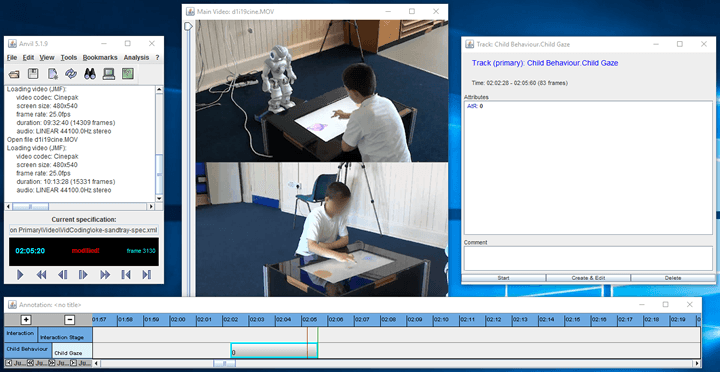
\includegraphics[width=1.0\textwidth]{images/ch3_anvil_comp.png}
    \caption{Screenshot of the ANVIL software package, showing \textit{clockwise} from the \textit{top-left}: (1) the menu, (2) the video player, (3) annotation panel, (4) coding/annotation time-line. Segments can be created on the time-line to indicate when behaviours occur.}
    \label{fig:ch3_anvil}
\end{figure}

All primary video coding performed in the experiments throughout this thesis was completed by the author. Video coding is an incredibly time consuming process, so second coding is done on a portion of the videos to provide some indication of reliability. Various second coders were used throughout the experiments, the majority of which were not aware of the experimental hypotheses. They were provided with a coding manual and a short training period before coding the videos intended for reliability checking. This methodology has been used elsewhere in \acrshort{hri} \citep{moshkina2014social}. The videos for second coding were pseudo-randomly selected; it was first ensured that an equal split between experimental conditions would be used, and then selected randomly to provide this balance. The quantity of videos for each experiment and the inter-rater agreement is specified as part of the methodological description within respective chapters where this analysis is performed.

%%%%%%%%%%%%%%%%%%%%%%%%%%%%%%%%%%%%%%%%%%%%%%%%%%%%%%%%%%%%
\section{Immediacy Questionnaires}\label{sec:method-nvi}
Chapter \ref{chap:background} introduced \textit{\gls{immediacy}} as a possible means of characterising robot social behaviour in \acrshort{hri}. Immediacy can be broken down into verbal and nonverbal aspects, each considering a different set of social cues. Questionnaires and scales for measuring both verbal and \gls{nonverbalimm} exist from the \acrshort{hhi} literature. Immediacy is used throughout the research in this thesis as a means of characterising social behaviour and to make comparisons between different experimental conditions. This section will discuss the \gls{immediacy} scales offered by the \acrshort{hhi} literature and how these were adapted for use with children, and for \acrshort{hri}.

The Nonverbal Immediacy Scale developed by \cite{richmond2003development} is the one typically adopted in most \acrshort{hhi} studies using \gls{immediacy} as a measure. However, there are multiple version of this scale available: observer report, self report, and short form (available online\footnote{\url{http://jamescmccroskey.com/measures/}}). The longer form versions contain 26 questions, whereas the short form version has 16 questions. These questions are all answered on a 5-point Likert scale (never, rarely, occasionally, often, very often) and contain both positively and negatively worded questions. The social cues considered include: touch, gaze, proximity, gesture, facial expression, and vocal prosody.

The \gls{verbalimm} scale is less widely agreed upon. \cite{gorham1988relationship} proposed and used a \gls{verbalimm} scale, which considers a series of \gls{verbalimm} behaviours specifically applied to teaching. This scale has been contested by \cite{robinson1995validity} who suggest that many of the items lack face validity with \gls{immediacy} as defined by \cite{mehrabian1968some}. Factor analysis of the whole \gls{immediacy} scale (verbal and nonverbal components combined) reveals that some of the verbal questions may not relate strongly to the \gls{immediacy} concept of psychological availability and should therefore be removed \citep{wilson2007immediacy}. However, the \gls{immediacy} measure is of interest here as a characterisation of social behaviour and because of the correlations found with learning. These correlations are found with the original version of the scale \citep{gorham1988relationship}. As such, the original version was used as a basis for the scale developed here. The \gls{verbalimm} items consist of a wide range of aspects of availability through spoken communication, such as the use of people's names, soliciting opinions, and discussing topics unrelated to any tasks being conducted. 

Immediacy scales are typically used with adults in lecture scenarios (e.g., \citealp{mccroskey1996nonverbal}) and the scales were developed in this context. As such, the linguistic abilities of children are not considered in the question wording. So that the scales can be used with children, the wording subsequently needs to be adapted. This wording adaptation was performed with the assistance of both a parent and a teacher of children of the age under consideration in this program of research. The full scales used can be seen in Appendices~\ref{app:rniq}, \ref{app:cniq} and \ref{app:riq}.

Where deemed necessary, the language used was simplified, and any abstractions were made more direct with the intention of making it apparent to the children that the questions were about their experience. So for example, ``he/she looks away from people while talking to them'' becomes ``the robot looks away from you while talking to you''. The layout of the scale was also modified; in the original versions statements are listed and the observer must place a rating from 1 to 5 before each statement. Due to concerns over interpreting children's handwriting and them remembering the number associated with each option, the options were placed after each question and simply required children to circle the answer that they wished to choose. Despite research which suggests an optimal number of options for children on a scale being four \citep{borgers2004response}, the five used in the original \gls{immediacy} scales were kept such that the overall \gls{immediacy} calculations and comparisons with prior literature could be maintained.

For the \gls{verbalimm} questionnaire, some questions were removed due to their irrelevance to the interaction context used in the research in later chapters. For example, ``invites students to meet or telephone after class...'' \citep{gorham1988relationship}, would not be appropriate given the context of the single interaction studies considered here.

%%%%%%%%%%%%%%%%%%%%%%%%%%%%%%%%%%%%%%%%%%%%%%%%%%%%%%%%%%%%
\section{Crowdsourcing Immediacy Ratings}\label{sec:method-crowdsource}
The work presented in subsequent chapters explores child learning and social behaviour in the context of various dyadic learning tasks, with different characters (be it physical embodiment, or behavioural differences). To create a common ground for comparison throughout these experiments, \gls{nonverbalimm} can be used to provide a characterisation of the social behaviour of the character that the children interact with.

In the case of experiments in subsequent chapters which explicitly manipulate \gls{immediacy}, immediacy ratings from the child participants are taken as part of the experimental protocol. In studies where \gls{immediacy} itself is not used to motivate behavioural comparisons, \gls{immediacy} ratings are not taken from the children, but it would nevertheless be desirable to have some measure of the \gls{nonverbalimm} in relation to behavioural manipulations for these studies. These ratings would allow all of the work throughout this thesis to be compared on the same scale, as well as providing greater context for the results on a per-study basis. These ratings were acquired post-hoc from adults due to the convenience of acquiring adult participants. Of course, this relies on adults perceiving \gls{nonverbalimm} in a similar way to children, as the child perception is the influencing factor for learning. This is investigated in Chapter \ref{chap:validation} (performed chronologically before the data collection described in this section to confirm validity of the approach before it was selected).

The \gls{nonverbalimm} ratings themselves are not presented or discussed here, but instead are incorporated as part of the discussion for each study as it appears in this document, as well as forming part of the larger framework in Chapter \ref{chap:behavemodel}. As such, the procedure is outlined here, and the data can be found in Appendix \ref{app:crowdsourced}. To provide sufficient subject numbers for all of the conditions, an online crowdsourcing service\footnote{\url{http://www.crowdflower.com/}} was used. Adults were shown short video clips from interactions with children and completed a \gls{nonverbalimm} questionnaire (Figure~\ref{fig:ch3_crowdsource_qs}). Details for the crowdsourcing procedure are outlined below.

\subsection{Quality Assurance}
To ensure the quality of the data collected from the crowdsourcing platform, a number of steps were taken in the creation of the crowdworker tasks, and in the verification of the data once it had been received. Some of these steps were automated through options within the crowdsourcing platform, whilst other checks were performed manually.

Using the crowdsourcing platform options, the participants were restricted to the USA and to English speakers in an effort to prevent too much variance due to cultural differences. The IP addresses of workers are monitored by the crowdsourcing platform for this purpose (so a determined worker could potentially still use a virtual private network to gain access to the job). Additionally, workers could only take part if they had a reliable record within the crowdsourcing platform. Specifically, only workers who had completed over 10 jobs and had no major flags, and up to 1 minor flag (flags refer to attempts to `cheat' jobs as judged by those creating the jobs) could participate. Due to these strict level requirements, and the consequence of workers losing access to other jobs, there is little incentive to attempt to cheat.

A test question was put in place in the job design whereby participants had to enter a 4 digit number into a text box (Figure~\ref{fig:ch3_crowdsource_vid}). This number was shown at the end of the video for 8 seconds (the video controls were disabled and the number would disappear after the video had finished). A different number was used for each video. If the participants did not enter this number correctly then their response was discarded. This was a means of identifying any workers attempting to answer the questions without having watched the whole video. This was to ensure the experimental protocol was being adhered to.

The crowdsourcing platform did not allow the prevention of users completing multiple conditions, so any duplicates were removed, i.e., only those seeing a video for the first time were kept as valid responses. This was a semi-automated step employed by the author after the data had been collected; a programming script was used to filter out all but the first job completed by any worker. A total of 496 responses were collected, but 266 were discarded as they did not answer the test question correctly, the user had completed another condition\footnote{The vast majority of exclusions were due to users having completed another condition.}, or the response was clearly spam (for example, all answers were `1'; this is a manual check by the author). One further response was excluded from analysis as it was an outlier (Grubbs' test). This left 229 responses across 7 conditions (Appendix~\ref{app:crowdsourced}).

\begin{figure}[ht]
    \centering
    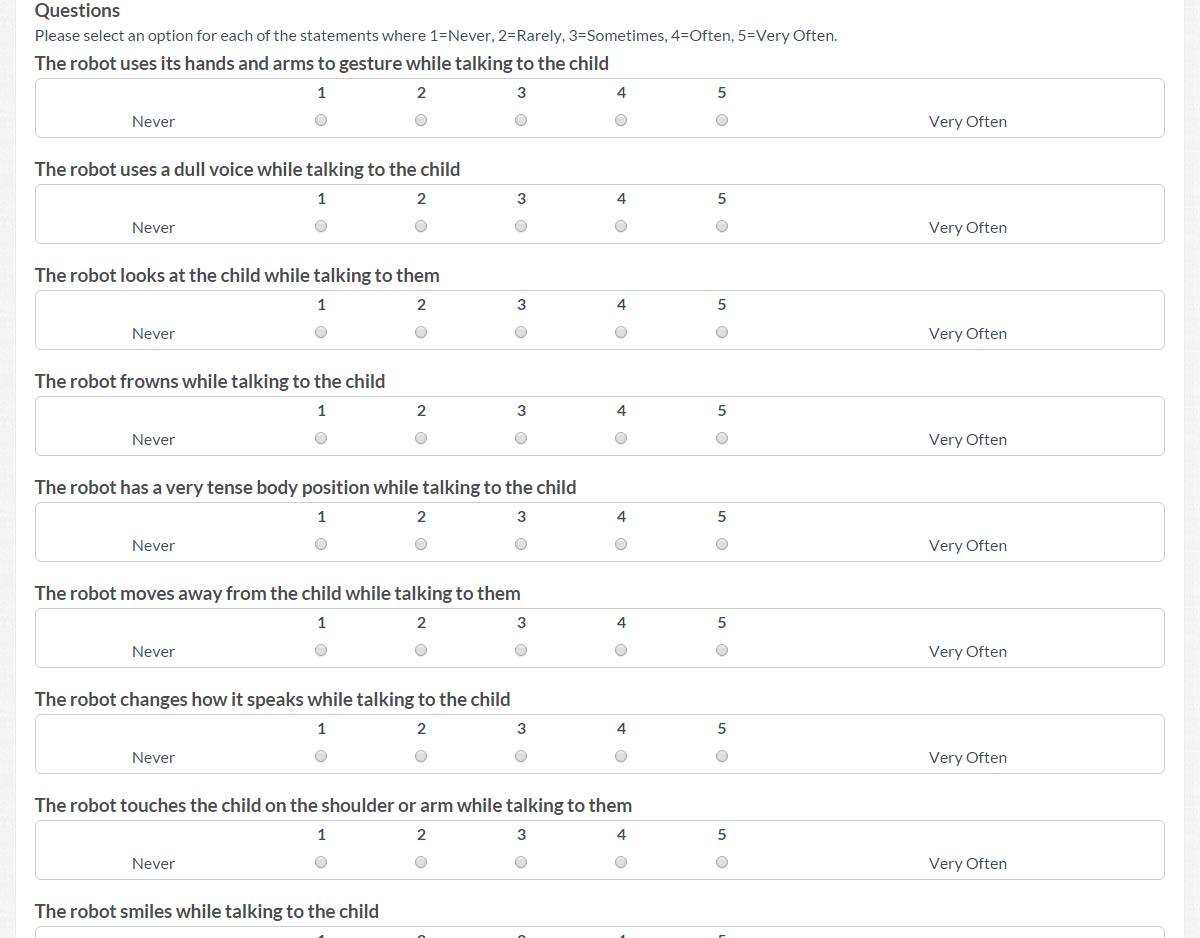
\includegraphics[width=0.9\textwidth]{images/ch3_crowdsource_qs.jpg}
    \caption{Screenshot from the online crowdsourcing service used to gather adult \gls{nonverbalimm} ratings. Radio boxes are used for answers to each question. The questionnaire is the same as that shown in Appendix \ref{app:rniq}, but with the language switched to be an observer report, rather than self-report (i.e., ``you'' is changed to ``the child'').}
    \label{fig:ch3_crowdsource_qs}
\end{figure}

\begin{figure}[ht]
    \centering
    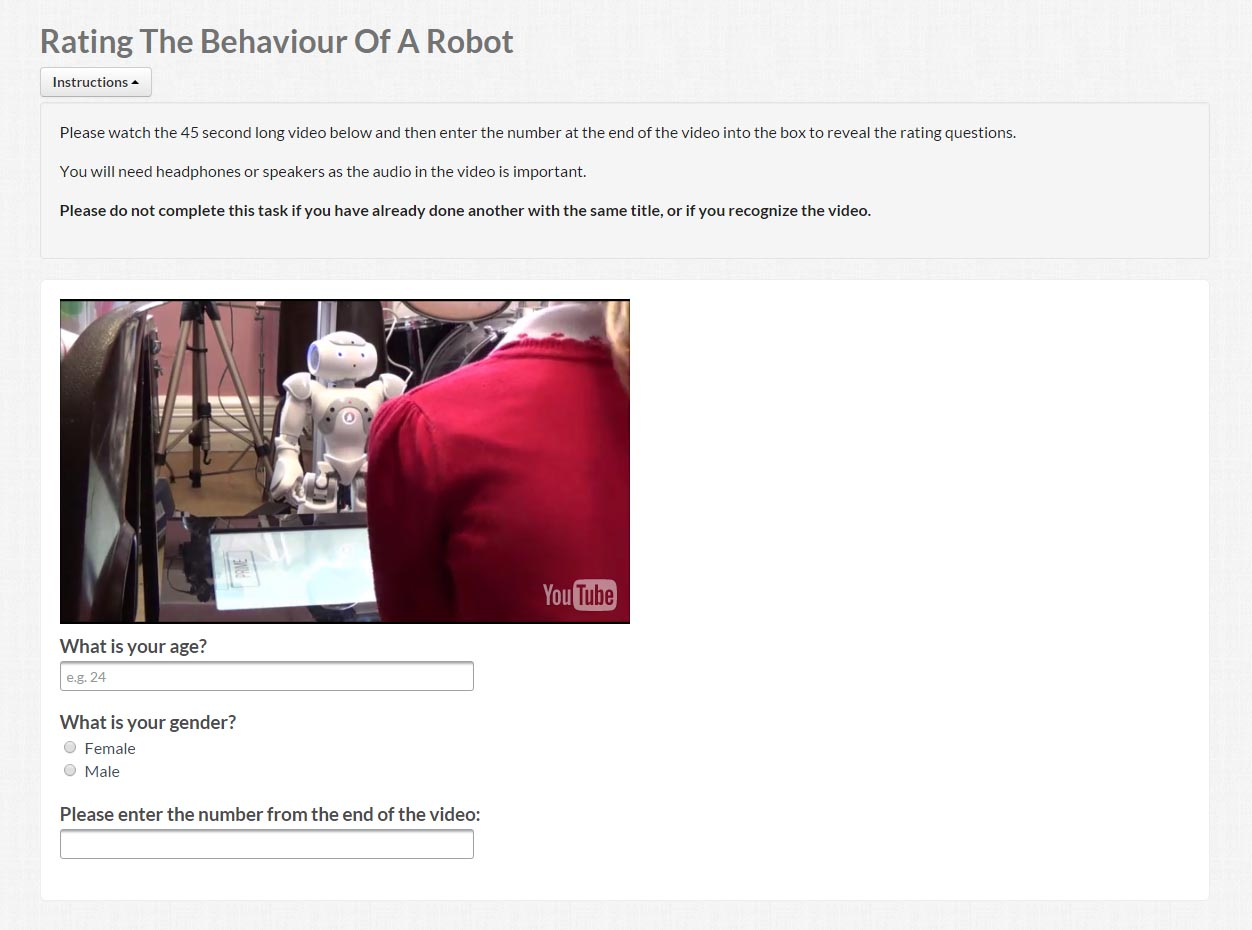
\includegraphics[width=0.9\textwidth]{images/ch3_crowdsource_vid.jpg}
    \caption{Screenshot from the online crowdsourcing service used to gather adult \gls{nonverbalimm} ratings. The video is embedded in the page, without controls. Nonverbal immediacy questions are not revealed until the number from the end of the video is entered, at which point the video is removed from the page.}
    \label{fig:ch3_crowdsource_vid}
\end{figure}

\subsection{Video and Questionnaire Format}
Videos shown to adults to acquire \gls{nonverbalimm} scores were each 47 seconds long. The videos contained both the interaction video (42 seconds) and a verification code (5 seconds; details in the following paragraph). The length of video was selected to be 42 seconds as the literature suggests that at least around 6-30 seconds are required to form a judgement of social behaviour \citep{ambady1993half} and there was a natural pause at 42 seconds in the speech in all conditions so that it wouldn't cut part-way through a sentence. The interaction clips were all from the start of an interaction, so the same information was being provided by the tutor to the child in the clip.

Only the \gls{nonverbalimm} scale was used as for \gls{verbalimm} responses to be accurate, the participants would need to have seen a much greater length of the video (possibly the full interaction) due to how often certain verbal behaviours occur and how long they last for. This would have placed a much greater strain on data collection; collecting over 200 opinions on a video of up to 15 minutes long is a much greater challenge than the same procedure when the video is 47 seconds long (which is still not straightforward). Additionally, in the majority of studies, verbal aspects of behaviour are constant between conditions, so a measure of the verbal behaviour is not as useful as a measure of the nonverbal behaviour. Where verbal behaviour is manipulated, child ratings for \gls{verbalimm} were collected (Chapter~\ref{chap:verbal}).

%%%%%%%%%%%%%%%%%%%%%%%%%%%%%%%%%%%%%%%%%%%%%%%%%%%%%%%%%%%%
\section{Practical Procedures}\label{sec:method-ethics}
Certain ethical considerations arise when conducting research with robots and children. These can be both general considerations that would be present when conducting research with children in any domain, and also domain specific. Many general considerations centre around the safety of the child and issues of consent. All of the experimental work conducted in this thesis was cleared by the university ethics board and adopts recommended best practices. This includes gaining consent from parents or guardians of children to conduct the research, but also informing the child of the nature of the research and providing them with the option to consent (or not) as well. To ensure child safety, they were always supervised when interacting with the robot, and no physical interaction between the child and the robot was present in any of the studies.

Domain specific ethical considerations consider those that relate either to children interacting with robots, or to the application of the research to child learning. Of course, there is an ethical responsibility to teach appropriate and correct material to the children. To this end, all of the work undertaken here was checked and approved by teachers. Some researchers have raised concerns over whether robots should be used to teach children at all (these broader aspects are explored further in Chapter \ref{chap:maindisc}). \cite{sharkey2016robot} presents several concerns related to the use of robots in classroom environments, including: privacy, deception, and reduced human contact. It is concluded that robots could offer new educational opportunities, but great care needs to be taken to prevent the robot from having a negative impact on child social relationships through loss of contact with other humans. The work conducted here primarily focusses on one-to-one tutoring for children, offering an addition to the current teaching environment, and certainly not a replacement for human teaching. Deception is kept to a minimum, partially through pursuit of autonomous, rather than `Wizarded' robot behaviours, and also through presenting the robot to all of the children after each study. In these presentations, the robot is described such that the children can see that the robot is a piece of technology, rather than an independent character, and they may ask any questions they have to the researcher. All data is kept anonymously and in accordance with university policy to protect the children's privacy.

When conducting experiments, effort was made to ensure that the children felt at ease not only interacting with the robot, but also with the experimenter(s). The class teacher would introduce the experimenters to the children on arrival at the school by their first name (as opposed to typical use of title and surname for adults in U.K. schools). The experimenters would inform the children about why they were visiting the school, and briefly set expectations for the children (for example, ``You will get to play a game with a robot that will teach you maths. All of you will have the chance to see the robot, so do not worry if you are not picked on the first day we are here.''). Further setting of child expectations was done by the experimenter immediately before the interaction; the experimenter would introduce the child to the robot and inform the child that the robot would tell them what they needed to do, whilst also making it known that they would be available if any problems arose, following advice from \citet{ros2011child}.

%%%%%%%%%%%%%%%%%%%%%%%%%%%%%%%%%%%%%%%%%%%%%%%%%%%%%%%%%%%%
\section{Summary}\label{sec:method-summary}
This chapter has introduced the materials used in the research in the later studies, specifically, the practical tools: the NAO robot, the Sandtray touchscreen, and the Microsoft Kinect. The various \gls{immediacy} questionnaires used have also been introduced, along with an explanation of the modifications made to make these questionnaires suitable for use with children and robots when compared to the originals used with adult humans. The processes involved in both video coding and adult crowdsourced \gls{nonverbalimm} ratings were also described.